\label{apendice:extra}

Após todos os experimentos analisados com os estados preditivos dos ativos, realizou-se então um novo experimento com informações de riscos fornecidas pelo \acrshort{MGR} sintético implementado. O experimentos foram realizados com parâmetros similares ao experimento de portfólio previamente realizado. Sua única diferença foi em relação ao estado do agente, agora o agente além de ter acesso a predição do ativo, tem acesso também ao indicador de riscos do \acrshort{MGR}.

Para cada ativo do portfólio, utiliza-se o volume de consultas do mesmo no \emph{Google Trends}. Esse volume representa a quantidade de pesquisas semanais entre $0$ a $100$ do termo pesquisado. No entanto, o \acrshort{MGR} processa essa informação, indicando um risco com o valor $1$ caso o valor esteja acima de um limite pré-determinado, ou $0$ caso o contrário. O experimento realizado possui um valor limite de $90$, representando que apenas pesquisas demasiadas indicariam um risco.

As \refFigs{all_risk_profit}{all_risk_act}, apresentam os resultados para o experimento. Como podemos ver, o experimento apresenta resultados semelhantes ao anterior (sem o \acrshort{MGR}). No entanto apresenta menos variações em seus resultados de teste em relação os valores encontrados sem o risco. O lucro encontrado é idêntico ao do experimento anterior, R\$$5.874,00$ no final do teste, uma rentabilidade de $11,74\%$ no total dos 6 meses. Sendo a única diferença aparente a impressão de uma conversão mais rápida ao resultado encontrado. Os outros gráficos obtidos durante o experimento foram omitidos por possuírem resultados muito similares ao experimento anterior. 

\begin{figure}[htbp]
    \centering 
    \begin{minipage}[b]{0.45\linewidth}
        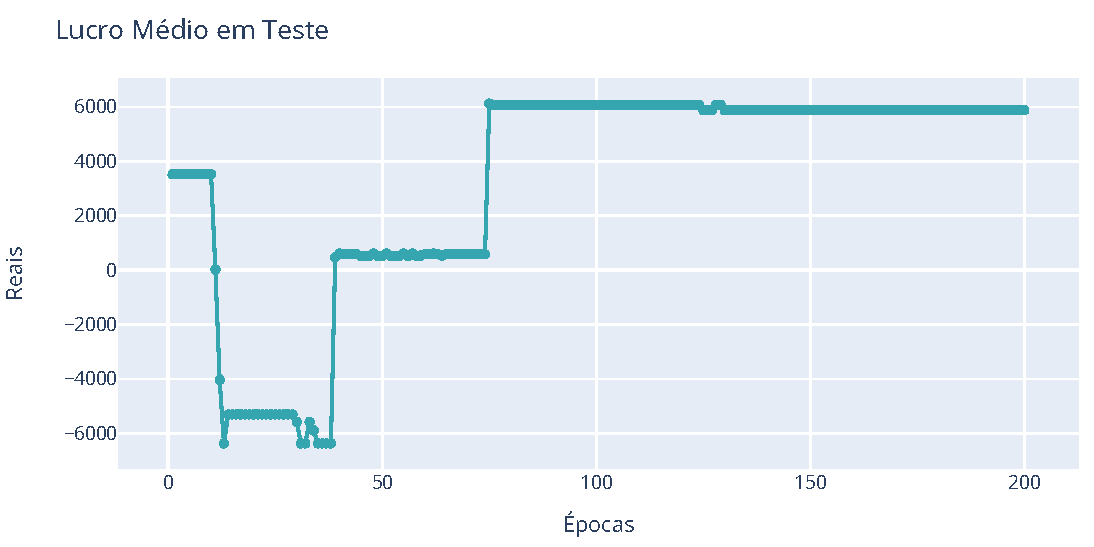
\includegraphics[width=\linewidth]{img/ddpg/all/risk/profit_test.pdf}
        \caption{Portfólio com \acrshort{MGR} - Lucro médio em teste.} 
        \label{all_risk_profit}
    \end{minipage}
    \quad
    \begin{minipage}[b]{0.45\linewidth}
        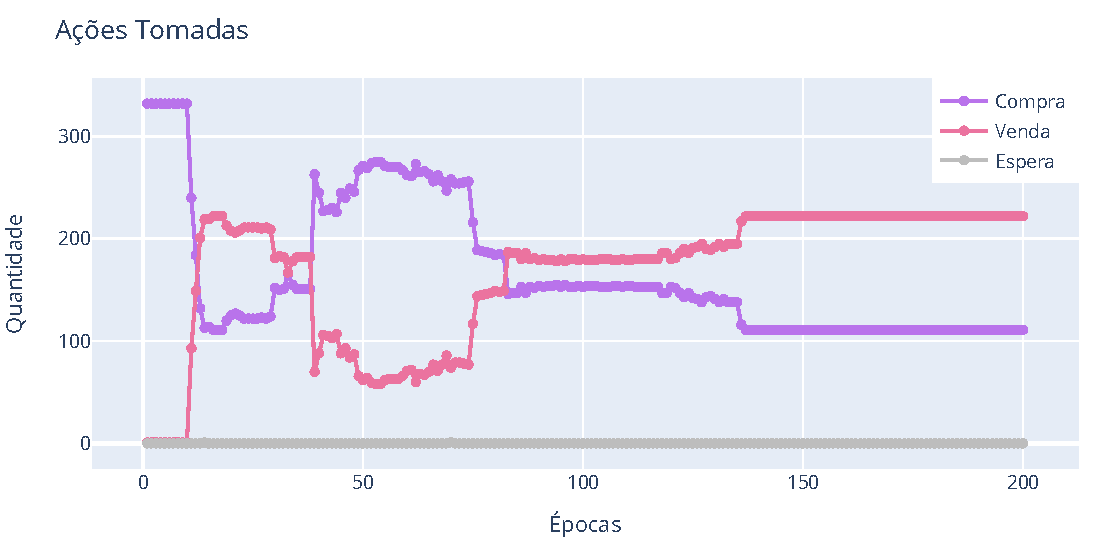
\includegraphics[width=\linewidth]{img/ddpg/all/risk/actions.pdf}
        \caption{Portfólio com \acrshort{MGR} - Quantidade de ações selecionadas.}
        \label{all_risk_act}
    \end{minipage}
\end{figure}

A semelhança dos resultados encontrados pode ser um indicativo de que o \acrshort{MGR} sintético não apresenta consistência em sua informação, e seguindo essa lógica de raciocínio, invalidaria a premissa de que um alto número de pesquisas representa necessariamente um risco. A implementação de modelos robustos para o \acrshort{MGR} e a análise mais profunda de seu comportamento será investigada em trabalhos futuros.